\chapter{Points, segments, droites, cercles et angles}

\activites

\begin{activite}[Segments, droites et demi-droites]

 \begin{partie}[À la découverte d'un nouveau code]
  \begin{enumerate}
   \item Lire la consigne de la case \circled{1} et observer la figure correspondant à cette consigne.
Faire de même pour la case \circled{2}.

Quand le code est compris, tracer la figure de la case \circled{3} et écrire la consigne de la case \circled{4}.


  \vspace{1em}
  
  
  
  \begin{tabular}{|c|c|c|c|c|}
  \cline{1-2}\cline{4-5}
    \circled{1} 		& \circled{2} 		& 	& \circled{3} 		& \circled{4}	\\ 
     Tracer $(AB)$ 	&  Tracer $[AC)$ 	& 	& Tracer $(AB)$	& 	 		\\ 
     Tracer $[AC]$ 	& Tracer $[BC]$ 	& 	& Tracer$[BC]$		& 			\\
     				&				&	& Tracer$[AC)$		&			\\ \cline{1-2}\cline{4-5}
   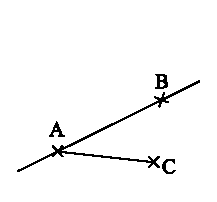
\includegraphics[width=.2\linewidth]{tracerAB-AC} & 
   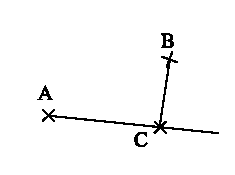
\includegraphics[width=.2\linewidth]{tracerAC-BC} & & 
   
\includegraphics[width=.2\linewidth]{tracerAB-BC-AC}& 
   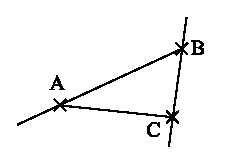
\includegraphics[width=.2\linewidth]{tracer} 					\\ \cline{1-2}\cline{4-5}
  \end{tabular}\\[1em]

  
   \item Lire la consigne de la case \circled{5} et observer la figure correspondant à cette consigne. Tracer ensuite la figure de la case \circled{6} et écrire la consigne de la case \circled{7}.
   
   \vspace{1em}
  
    \begin{tabular}{|l|l|l|}
   \hline
    \hfill \circled{5} \hfill			&	\hfill \circled{6} \hfill				&	\hfill \circled{7} \hfill 	\\
    - Tracer la droite passant par 	&	- Tracer le segment 				&					\\
    $E$ et $F$ ;					&	d'extrémités $R$ et $S$ ;			&					\\
    - Tracer le segment 			&	- Tracer la droite passant par 		&					\\
    d'extrémités $E$ et $G$ ;		&	$R$ et $T$ ;					&					\\
    - Tracer la demi-droite 			&	- Tracer la demi-droite 			&					\\
    d'origine $G$ et passant par $F$.	&	d'origine $S$ et passant par $T$.	&					\\ \hline
    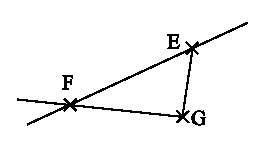
\includegraphics[width=.24\linewidth]{tracerEFG} 			&  
    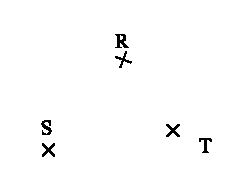
\includegraphics[width=.24\linewidth]{tracerRST}			&
    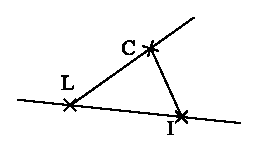
\includegraphics[width=.24\linewidth]{tracerLCI}			\\ \hline
    \end{tabular}\\[1em]

    
  \newpage
  
   \item Compléter le tableau suivant :
   
   \vspace{1em}
   
   \renewcommand*\tabularxcolumn[1]{>{\centering\arraybackslash}m{#1}}
   \begin{ttableau}{\linewidth}{3}
    \hline
    \multicolumn{1}{|c|}{\textbf{Phrase}}	&	\multicolumn{1}{c}{\textbf{Phrase codée}}	&	\multicolumn{1}{|c|}{\textbf{Dessin}}			 	\\  \hline
    								&	Tracer $[UV]$							&	
\includegraphics[width=2.6cm]{phraseUV}		\\  \hline
    								&										&	
\includegraphics[width=3.2cm]{phraseAM}		\\  \hline
   Tracer la droite passant par $S$ et $T$	&										&	
\includegraphics[width=2.6cm]{phraseST}		\\  \hline
   								&										&	
\includegraphics[width=4.0cm]{phraseAM_2}	\\  \hline
   Tracer le segment d'extrémités $M$ et $N$	&									&	
\includegraphics[width=2.6cm]{phraseMN} 	\\  \hline
   								&	Tracer $[KJ)$							&	
\includegraphics[width=2.6cm]{phraseKJ}		\\  \hline
								&										&	
\includegraphics[width=2.6cm]{phraseAM_3}	\\  \hline
   Tracer la demi-droite d'origine $O$ et 	&										&	
\includegraphics[width=2.6cm]{phraseOU}		\\
   passant par $U$					&										&										\\  \hline
   								&	Tracer $(BC)$							&	
\includegraphics[width=2.6cm]{phraseBC}		\\  \hline
  \end{ttableau}
  
   \end{enumerate} 

  \end{partie}

\end{activite}

\newpage

%%%%%%%%%%%%%%%%%%%%%%%%%%%%%%%%%%%%%%%%%%%%%

\begin{activite}[Repérer des droites perpendiculaires]

 \begin{minipage}[c]{0.50\linewidth}
  \begin{partie}[Éric a oublié son équerre !]
 
  « Pas de souci, lui dit son professeur, prends une feuille blanche non quadrillée. Tu devrais pouvoir obtenir un angle droit en pliant deux fois cette feuille. »
  
  Réalise une telle équerre.
  
  Qu'obtiens‑tu si tu déplies ta feuille ? 
    \end{partie}
  
  \begin{partie}[Éric utilise sa nouvelle équerre \ldots]
  
  Éric doit replacer l'équerre dans la position qui a permis de construire les droites $d_4$ et $d_7$. \\[0.5em]
  Place l'équerre dans cette position. \\[0.5em]
  Trouve alors un autre couple de droites \textbf{perpendiculaires} sur cette figure en t'aidant de ton équerre.
    \end{partie} \end{minipage} \hfill %
   \begin{minipage}[c]{0.44\linewidth}
   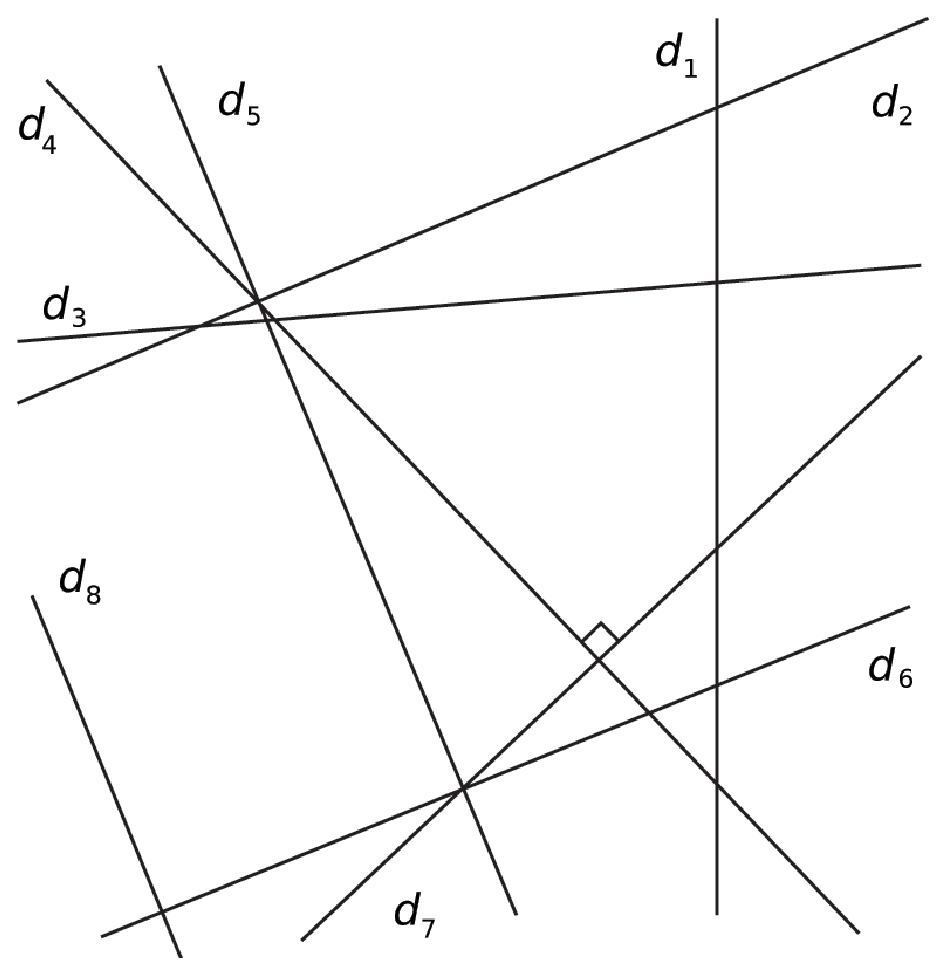
\includegraphics[width=6.1cm]{plusieurs_droites}
   \end{minipage} \\

 \begin{partie}[Utilisation de l'équerre d'Éric]
 
Trace deux droites sécantes $d$ et $d'$. À l'aide de l'équerre que tu as fabriquée, construis une droite perpendiculaire à $d$ et une autre perpendiculaire à $d'$. Tu n'oublieras pas d'ajouter les codages nécessaires.

  \end{partie} 
  
\end{activite}

%%%%%%%%%%%%%%%%%%%%%%%%%%%%%%%%%%%%%%%%%%%%%

\begin{activite}[Droites parallèles]

 \begin{partie}[Deux droites perpendiculaires]
 
  \begin{enumerate}
   \item Place deux points $A$ et $B$.
   \item Trace une droite $d$ ne passant ni par $A$, ni par $B$ et qui coupe $(AB)$.
   \item Trace $d_1$ la perpendiculaire à d passant par $A$, puis la droite $d_2$ perpendiculaire à $d_1$ passant par $B$. Que remarques‑tu ?
   \item Trace $d_3$ la perpendiculaire à $d$ passant par $B$ et $d_4$ la perpendiculaire à $d_3$ passant par $A$. Que peux‑tu dire de $d_2$ et $d_4$ ? Quelles autres remarques du même type peux‑tu faire ? 
   \end{enumerate}
   
  \end{partie} 

 \begin{partie}[Construction à la règle et à l'équerre]
 
 \begin{minipage}[c]{0.66\linewidth}
 La première vignette d'une bande dessinée est représentée ci‑contre. On y a placé une droite $d$ et un point $A$ n'appartenant pas à $d$.
 Complète cette bande dessinée pour expliquer comment, à l'aide de la règle et de l'équerre, tu traces la \textbf{parallèle} à $d$ passant par $A$.
  \end{minipage} \hfill %
 \begin{minipage}[c]{0.3\linewidth}
 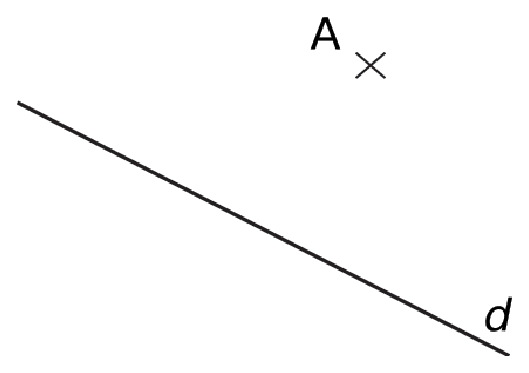
\includegraphics[width=4.2cm]{droiteAd}
  \end{minipage} \\
 
  \end{partie} 

\end{activite}

%%%%%%%%%%%%%%%%%%%%%%%%%%%%%%%%%%%%%%%%%%%%%

\begin{activite}[Tout savoir sur la médiatrice !]

 \begin{partie}[Axes de symétrie d'un segment]
 
 \begin{enumerate}
  \item Sur une feuille blanche, trace un segment $[AB]$.
  \item Plie cette feuille de manière à ce que le point $A$ touche le point $B$, cela fait apparaître un axe de symétrie de ce segment. Le symétrique de $A$ par rapport à cet axe est $B$. Comment s'appelle cet axe ? Repasse‑le en couleur.
  \item Quelles sont ses caractéristiques ?
  \end{enumerate}
  
  \end{partie}
  
 \begin{partie}[Propriété d'un point appartenant à la médiatrice d'un segment]
 
 \begin{enumerate}
  \item Place un point $M$ sur cette médiatrice. Que dire des longueurs $AM$ et $BM$ ?
  \item Que dire alors d'un point qui appartient à la médiatrice d'un segment ?
  \end{enumerate}
  
  \end{partie}
  
 \begin{partie}[Ensemble de points]
 
 \begin{minipage}[c]{0.76\linewidth}
 \begin {enumerate}
  \item Construis un segment $[CD]$ de longueur 5 cm. 
  \item Place $A$, \textbf{équidistant} de $C$ et de $D$. Place trois autres points équidistants de $C$ et de $D$. 
  \item Où semblent se trouver tous les points équidistants de $C$ et $D$ ?
  \item Que dire d'un point équidistant des extrémités d'un segment ?
  \item Déduis‑en une façon de construire la médiatrice d'un segment sans l'équerre. 
  \end{enumerate} 
  \end{minipage} \hfill %
 \begin{minipage}[c]{0.2\linewidth}
 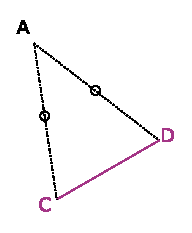
\includegraphics[width=2.8cm]{triangleACD}
  \end{minipage} \\
  
 \end{partie}

\end{activite}

%%%%%%%%%%%%%%%%%%%%%%%%%%%%%%%%%%%%%%%%%%%%%

\begin{activite}[Bissectrice, qui es-tu ?]

 \begin{partie}[Définition] \label{EntDroitSeg_DefBissectrice}

 \begin{minipage}[c]{0.68\linewidth}
 \begin {enumerate}
  \item Sur une feuille blanche, trace un angle $\widehat{ABC}$.
  \item Plie cette feuille de façon à faire apparaître l'axe de symétrie de l'angle. Repasse‑le en couleur. Place un point D sur cet axe (comme sur le croquis ci contre). \label{EntDroitSeg_plier}
  \item Cet axe fait apparaître deux nouveaux angles. Nomme‑les.
  \item Que peut‑on dire de la mesure de ces deux angles ? Justifie. Comment nomme‑t‑on cette droite ?
  \end{enumerate} 
  \end{minipage} \hfill %
 \begin{minipage}[c]{0.26\linewidth}
 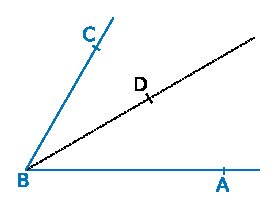
\includegraphics[width=3.8cm]{bissectrice}
  \end{minipage} \\
  
 \end{partie}
 
 \begin{partie}[Construction au compas]
 
 \begin{enumerate}
 \item Construis le point $A'$ symétrique du point $A$ par rapport à la bissectrice de l'angle $\widehat{ABC}$ Tu obtiens ce point en reportant le point A sur la droite $[BC)$ en pliant la feuille comme au point \ref{EntDroitSeg_plier} de la partie \ref{EntDroitSeg_DefBissectrice}. Que dire des longueurs $BA$ et $BA'$ ?
 \item Que représente la bissectrice de l'angle $\widehat{ABC}$ pour le segment $[AA']$ ?
 \item Déduis‑en une façon de construire la bissectrice d'un angle sans rapporteur.
  \end{enumerate}              
  \end{partie}
 
\end{activite}

%%%%%%%%%%%%%%%%%%%%%%%%%%%%%%%%%%%%%%%%%%%%%

\begin{activite}[De qui est-ce la trace ?]

 \begin{partie}
 Sur ton cahier, place un point $O$. Recherche tous les points situés à 3 cm du point $O$. 
  \end{partie}

 \begin{partie}
 \begin{minipage}[c]{0.78\linewidth}
 Un système d'arrosage automatique est formé d'un jet qui arrose dans toutes les directions jusqu'à 4 m.
  \begin {enumerate}
  \item Représente sur ton cahier la zone arrosée par le jet en appelant $J$ l'emplacement du jet. (1 cm représentera 1 m.)
  \item Comment peux‑tu définir les points de la zone arrosée ? 
  \end{enumerate} 
  \end{minipage} \hfill %
 \begin{minipage}[c]{0.16\linewidth}
 
\includegraphics[width=2cm]{arrosage}
  \end{minipage} \\
    
  \end{partie}

\end{activite}

%%%%%%%%%%%%%%%%%%%%%%%%%%%%%%%%%%%%%%%%%%%%%

\begin{activite}[Des constructions]

 \begin{partie}[Du programme à la figure]
 Réalise la suite d'instructions suivantes :
 \begin{itemize}
  \item Trace un cercle $(\mathcal{C})$ de centre $O$ et de rayon 5 cm.
  \item Place, sur le cercle, deux points $A$ et $B$ \textbf{diamétralement opposés}.
  \item Construis le cercle $(\mathcal{C}_1)$ de diamètre $[OA]$ et le cercle $(\mathcal{C}_2)$ de diamètre $[OB]$.
  \item Trace le cercle $(\mathcal{C}_3)$ de centre $A$ passant par $O$.
  \item Nomme $E$ et $F$ les \textbf{points d'intersection} des cercles $(\mathcal{C})$ et $(\mathcal{C}_3)$.
  \item Trace le cercle $(\mathcal{C}_4)$ de centre $B$ et de rayon $OB$.
  \item Les cercles $(\mathcal{C})$ et $(\mathcal{C}_4)$ se coupent en $G$ et $H$.
  \end{itemize}
  
  \end{partie}
  
  \vspace{2em}
  
 \begin{partie}[De la figure au programme]
 \begin{minipage}[c]{0.48\linewidth} 
Construis la figure ci‑contre donnée 

par son croquis.

Écris le programme de construction.
 \end{minipage} \hfill %
 \begin{minipage}[c]{0.46\linewidth}
 
\includegraphics[width=4.2cm]{figure-programme}
  \end{minipage} \\
  
  \end{partie}

\end{activite}

%%%%%%%%%%%%%%%%%%%%%%%%%%%%%%%%%%%%%%%%%%%%%


\cours
\section{Les angles}

%%%%%%%%%%%%%%%%%%%%%%%%%%%%%

% remarque : pour qu'un mot se retrouve dans le lexique : \MotDefinition{asymptote horizontale}{} 

\begin{definition}
Un \MotDefinition{angle}{} est une portion de plan délimitée par deux demi-droites ayant la même origine.
 \end{definition}

\subsection{Reconnaître les différents types d'angles}

On classe les angles par catégories selon leur mesure.

 \renewcommand*\tabularxcolumn[1]{>{\centering\arraybackslash}m{#1}}
 \begin{ttableau}{\linewidth}{6}
\hline \textbf{Angle} 	&	Nul	&	Aigu		&	Droit		&	Obtus	&	Plat	\\ \hline
 \textbf{Figure} 	&	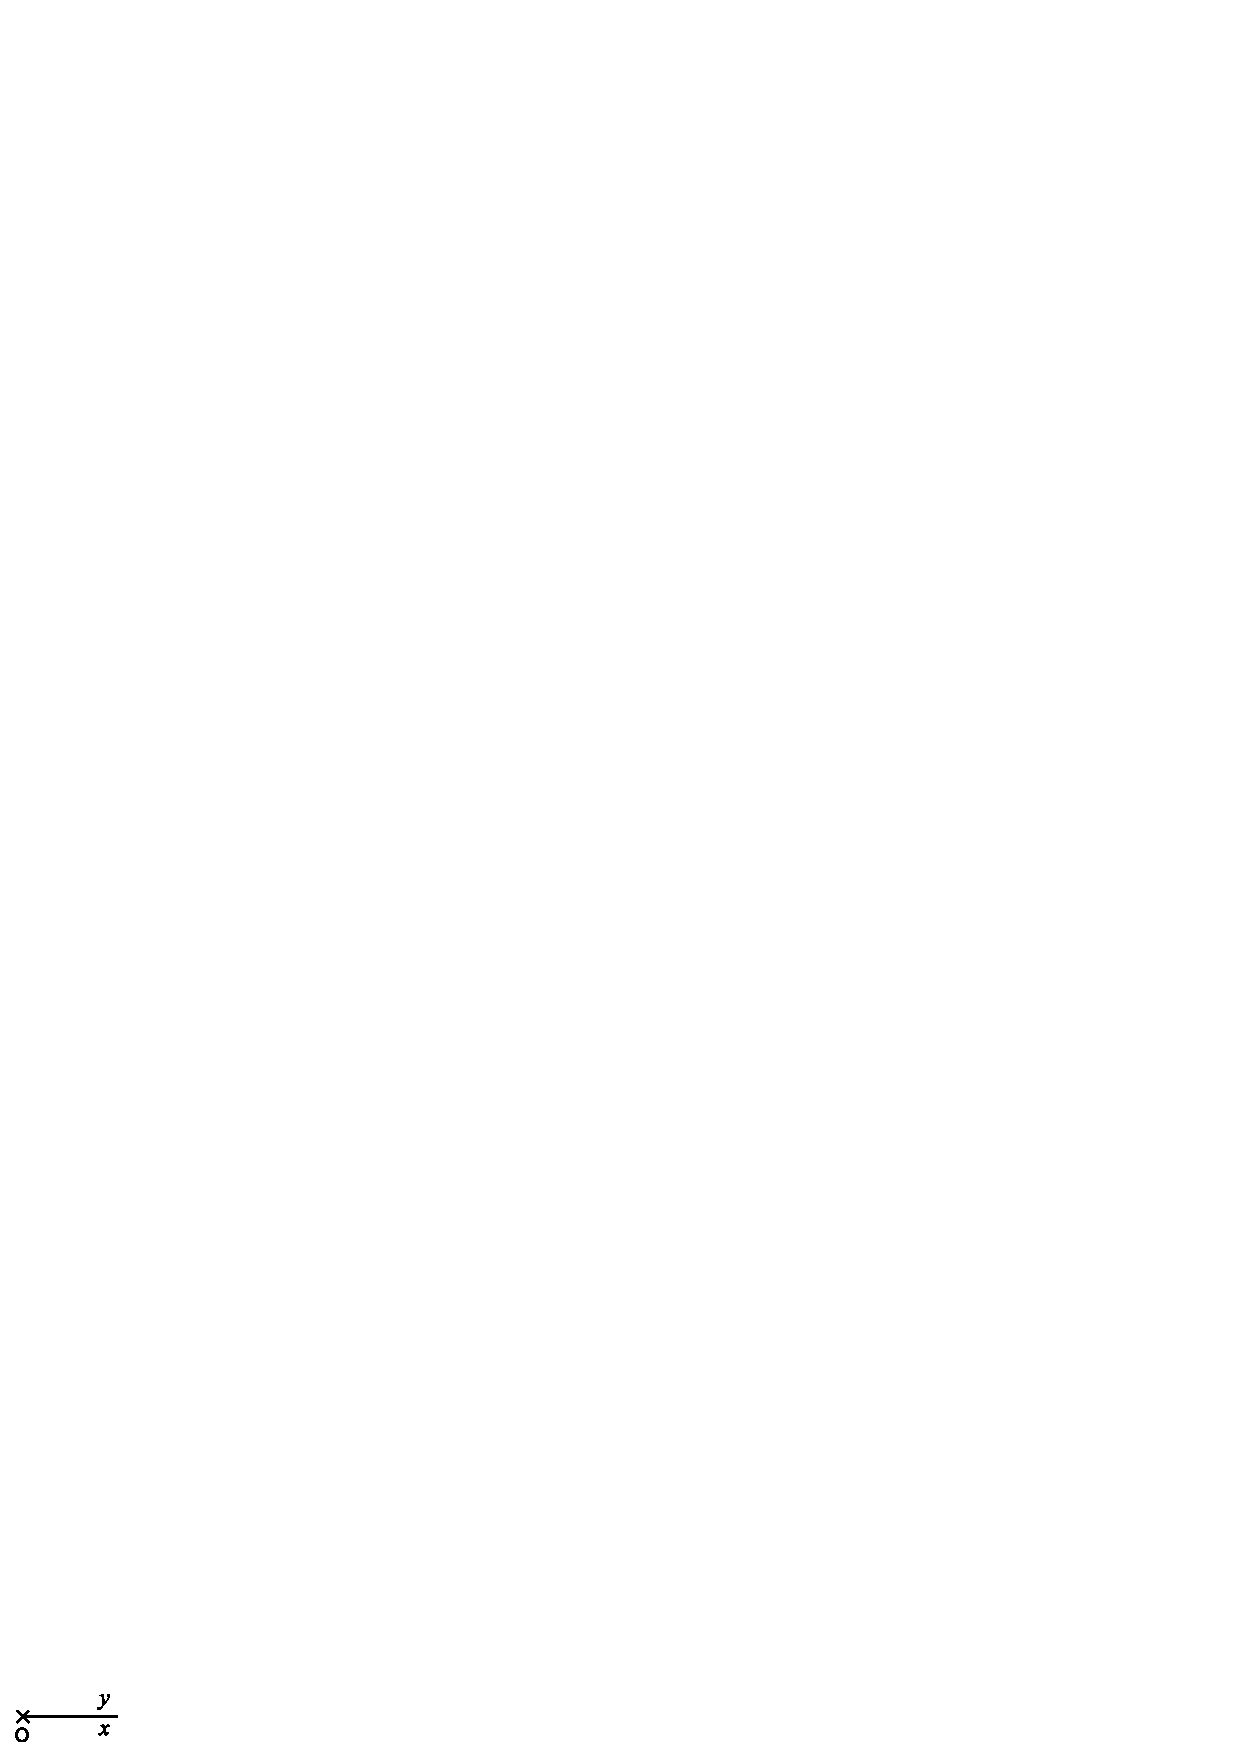
\includegraphics[width=1.7cm]{angle_nul}	&	
\includegraphics[width=1.7cm]{angle_aigu}	&	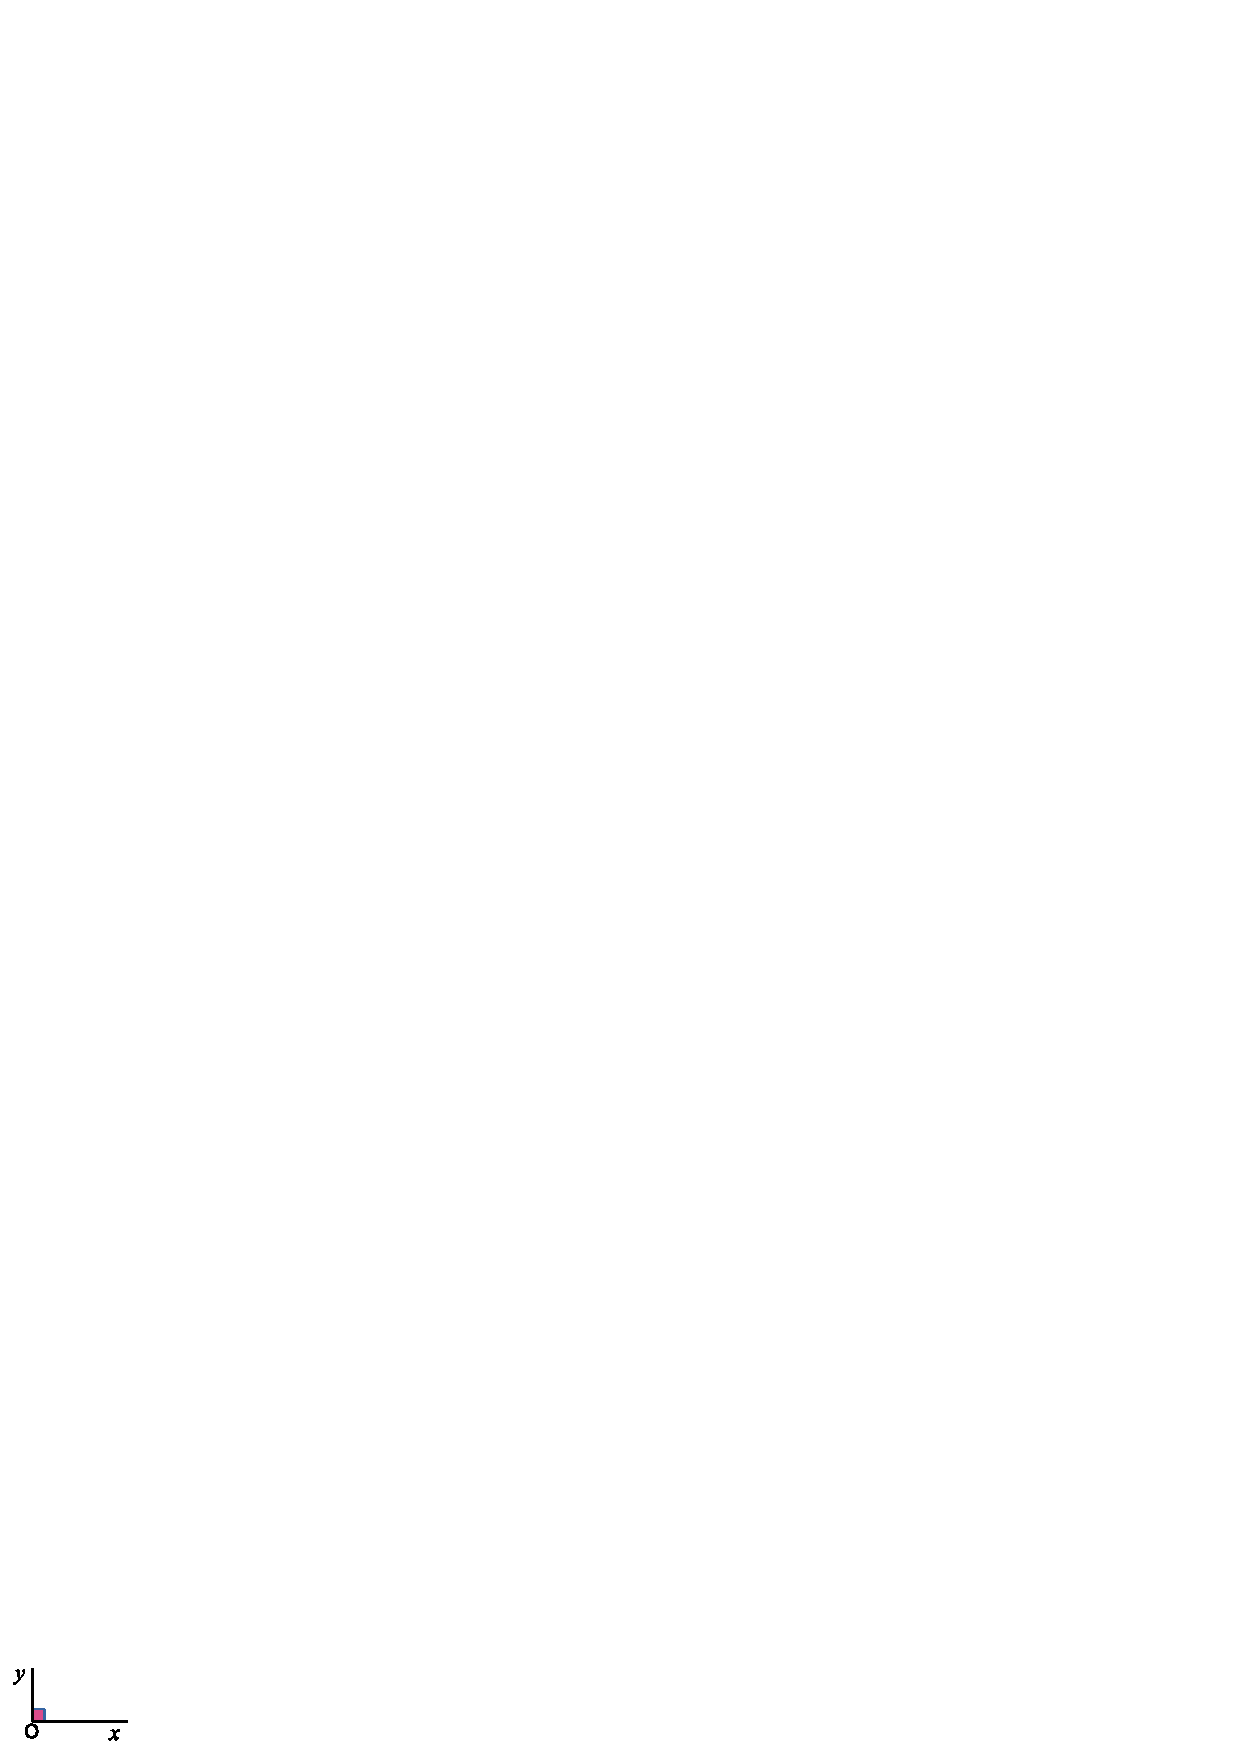
\includegraphics[width=1.7cm]{angle_droit}	&	
\includegraphics[width=1.7cm]{angle_obtus}	&	
\includegraphics[width=1.7cm]{angle_plat}	\\ \hline
 \textbf{Mesure} 	&	$0^\circ$	&	entre $0^\circ$ et $90^\circ$	&	$90^\circ$		&	entre $90^\circ$ et $180^\circ$	&	 $180^\circ$	\\ \hline
 \multirow{3}{*}{\textbf{Position des côtés}} 	&		&	&	&	&	dans le 	\\ 
 	&	confondus		&	&	perpendiculaires	&	&	 prolongement	\\
	&	&	&	&	&	 l'un de l'autre	\\ \hline
 \end{ttableau}

%%%%%%%%%%%%%%%%%%%%%%%%%%%%%

\begin{methode*1}[Nommer un angle]

\begin{exemple*1}
Nomme l'angle marqué en violet sur la figure ci‑dessous.  \\[0.75em]

\begin{minipage}[c]{0.70\textwidth}
Le sommet de l'angle est le point $C$ : c'est la lettre centrale. \\[0.5em]
Les côtés de l'angle sont les demi‑droites $[CH)$ (ou $[Cx)$) et $[CS)$ (ou $[CA)$ (ou $[Cy)$). \\[0.5em]
Cet angle peut se nommer : $\widehat{{\textcolor{A1}{H}}C{\textcolor{C1}{S}}}$; $\widehat{{\textcolor{C1}{S}}C{\textcolor{A1}{H}}}$ ; $\widehat{{\textcolor{A1}{H}}C{\textcolor{C1}{A}}}$ ; $\widehat{{\textcolor{C1}{A}}C{\textcolor{A1}{H}}}$ ; $\widehat{{\textcolor{C1}{y}}C{\textcolor{A1}{x}}}$.
 \end{minipage} \hfill%
 \begin{minipage}[c]{0.26\textwidth}
 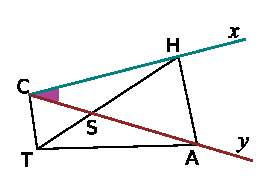
\includegraphics[width=3.8cm]{nommer_angle}
 \end{minipage} \\
 
\end{exemple*1}

\exercice 
Nomme les angles marqués sur la figure ci‑dessous. 
\begin{center} 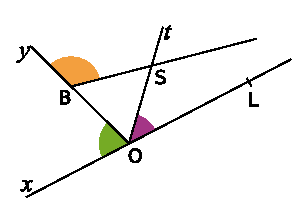
\includegraphics[width=4.5cm]{nommer_angles} \end{center}
%\correction
 
\end{methode*1}

%%%%%%%%%%%%%%%%%%%%%%%%%%%%%

\begin{methode*1}[Utiliser le rapporteur]

\begin{exemple*1}
Mesure l'angle $\widehat{CAB}$. \\[0.75em]

\begin{minipage}[c]{0.49\textwidth}
\centering
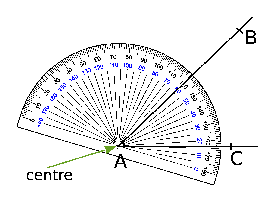
\includegraphics[width=4.8cm]{rapporteur1}
\end{minipage}\hfill%
 \begin{minipage}[c]{0.49\textwidth}%
 \centering
 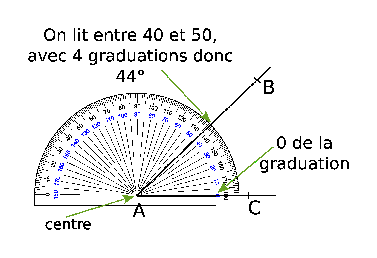
\includegraphics[width=6.6cm]{rapporteur2}
  \end{minipage} \\
 \begin{minipage}[c]{0.43\textwidth}
On place le centre du rapporteur sur le sommet de l'angle.
\end{minipage} \hfill%
 \begin{minipage}[c]{0.53\textwidth}
 On place un zéro du rapporteur sur le côté $[AC)$. Si besoin, on prolonge la demi‑droite $[AC)$. La mesure de l'angle est donnée par l'autre côté de l'angle sur \underline{la même échelle} de graduation.
 \end{minipage} \\
  \end{exemple*1}
 
 \begin{exemple*1}
Construis un angle $\widehat{BUT}$ de $108^\circ$.  \\[0.75em]

\begin{minipage}[c]{0.49\textwidth}
\centering
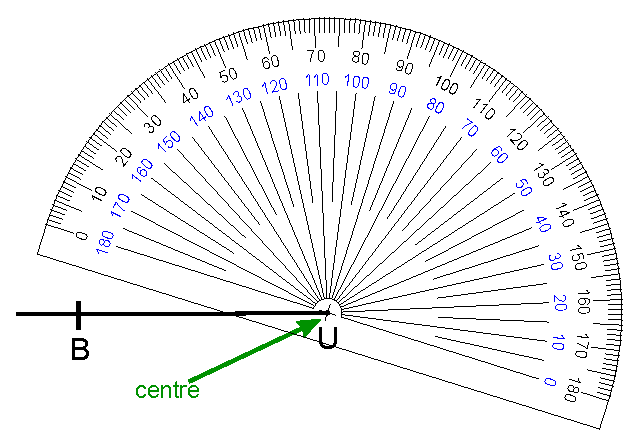
\includegraphics[width=4.8cm]{rapporteur3}
\end{minipage}\hfill%
 \begin{minipage}[c]{0.49\textwidth}%
 \centering
 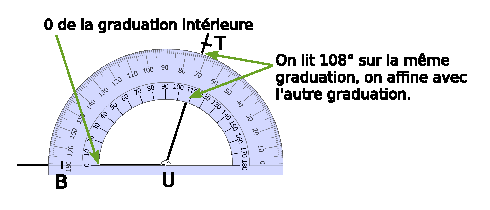
\includegraphics[width=6.6cm]{rapporteur4}
  \end{minipage} \\
 \begin{minipage}[c]{0.43\textwidth}
On trace $[UB)$, premier côté de l'angle. On place le centre du rapporteur sur le point $U$.
\end{minipage} \hfill%
 \begin{minipage}[c]{0.53\textwidth}
 On place un zéro du rapporteur sur le côté $[UB)$. On marque, d'un petit trait-repère, $108^\circ$ avec la bonne graduation.
On trace la demi‑droite d'origine $U$ passant par le repère. On place un point $T$ sur cette demi‑droite.
  \end{minipage} \\
  \end{exemple*1}
 
\exercice
 \begin{enumerate}
 \begin{minipage}[c]{0.36\textwidth}
  \item Mesure l'angle $\widehat{xOy}$ ci‑contre ;
  \item Construis un angle $\widehat{SAT}$ de $85^\circ$. 
  \end{minipage} \hfill%
 \begin{minipage}[c]{0.56\textwidth}
  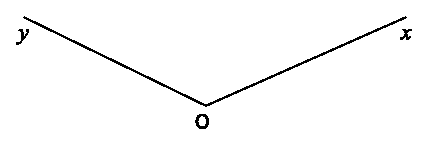
\includegraphics[width=6cm]{angleyOx} 
  \end{minipage} \\
  \end{enumerate}
%\correction
 
\end{methode*1}

%%%%%%%%%%%%%%%%%%%%%%%%%%%%%

\section{Constructions graphiques : parallèles et perpendiculaires}

\begin{methode*1}[Construire la perpendiculaire à une droite passant par un point]

\begin{exemple*1}
Trace une droite $d$ et place un point $M$ n'appartenant pas à la droite $d$.

Trace la droite $d'$ perpendiculaire à la droite $d$ passant par le point $M$. \\[0.75em]

\begin{tabularx}{\textwidth}{X|X|X|X}
 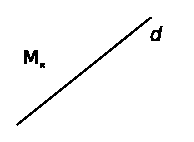
\includegraphics[width=2.4cm]{droiteMxd} &  
\includegraphics[width=2.4cm]{equerre} & 
\includegraphics[width=2.4cm]{regle} &  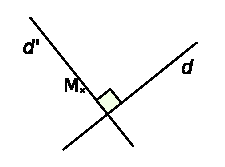
\includegraphics[width=2.4cm]{angledMd}\\ 
 On trace une droite $d$ et on place un point $M$. & On place l'un des côtés de l'angle droit de l'équerre sur la droite $d$ et l'autre côté sur $M$.
 & On prolonge la droite à la règle. & On nomme la droite $d'$ et on code l'angle droit par un carré.\\

\end{tabularx} \\
 
 \end{exemple*1}


\exercice

En utilisant cette méthode, tracer un rectangle ABCD de longueur 3 cm et de longueur 5 cm.

%\correction

 
\end{methode*1}

\newpage

%%%%%%%%%%%%%%%%%%%%%%%%%%%%%

\begin{methode*1}[Construire la parallèle à une droite passant par un point]

\begin{exemple*1}
Trace une droite $d$ et place un point $M$ n'appartenant pas à la droite $d$.

Trace la droite $d'$ parallèle à la droite $d$ passant par le point $M$. \\[0.75em]

\begin{tabularx}{\textwidth}{X|X|X|X}
 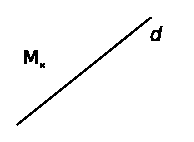
\includegraphics[width=2.4cm]{droiteMd} &  
\includegraphics[width=2.4cm]{equerreMd} & 
\includegraphics[width=2.4cm]{equerre_regle} &  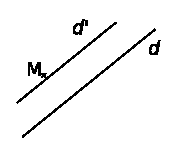
\includegraphics[width=2.4cm]{2droites}\\ 
On trace une droite $d$ et on place un point $M$. & On place l'un des côtés de l'angle droit de l'équerre sur la droite $d$. & On fait coulisser l'équerre le long de la règle, jusqu'au point $M$, sans bouger la règle. & On trace ainsi la droite $d'$.\\
\end{tabularx} \\
 
 \end{exemple*1}

\exercice 
Trace dans ton cahier un segment $[AB]$ d'une longueur de 5 cm et place un point $C$ au-dessus du segment $[AB]$ ($C$ n'est pas sur le segment). Construis, en rouge, la perpendiculaire à $[AB]$ passant par $C$. Construis, en vert, la parallèle à $[AB]$ passant par $C$.
%\correction

\end{methode*1}

%%%%%%%%%%%%%%%%%%%%%%%%%%%%%
\newpage

\section{La médiatrice}

\begin{definition}
La \textbf{\MotDefinition{médiatrice}{}} d'un segment est la droite qui coupe ce segment perpendiculairement en son milieu.
\end{definition}


\begin{methode*1}[Construire une médiatrice]

\begin{exemple*1}
Trace un segment $[OS]$ de longueur 5 cm puis sa médiatrice. \\[0.75em]

\begin{tabularx}{\textwidth}{X|X|X|X}
 
\includegraphics[width=2.4cm]{segmentOS} &  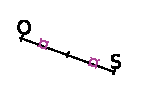
\includegraphics[width=2.4cm]{milieu_segmentOS} & 
\includegraphics[width=2.4cm]{segmentOS_equerre} &  
\includegraphics[width=2.4cm]{segmentOS_droit} \\ 
On trace un segment $[OS]$. & On trace le milieu du segment. & On trace la droite perpendiculaire au segment qui passe par ce milieu. & On code l'angle droit par un carré. \\
\end{tabularx} \\

 \end{exemple*1}
 
 \begin{exemple*1}
Trace un segment $[AB]$ de longueur 6 cm. Construis sa médiatrice au compas. \\[0.75em]

\begin{tabular}{l|l|l|l}
 \textcolor{H1}{\circled{1}} &  \textcolor{H1}{\circled{2}} &  \textcolor{H1}{\circled{3}} & \textcolor{H1}{\circled{1}} On trace le segment $[AB]$. \\ 
 \multirow{7}{*}{
\includegraphics[width=2cm]{regleA}} &  \multirow{7}{*}{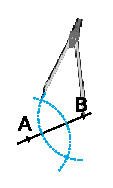
\includegraphics[width=1.5cm]{compasAB}} & \multirow{7}{*}{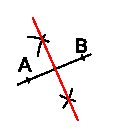
\includegraphics[width=1.5cm]{mediatriceAB}} &  \textcolor{H1}{\circled{2}} On trace deux arcs de cercle de \\ % exemple de fusion de cellules d'une même colonne
&&&  centres $A$ et $B$, de même rayon \\ 
&&& en choisissant un rayon \\
&&& suffisamment grand pour que ces \\
 &&& arcs se coupent en deux points. \\
&&& \textcolor{H1}{\circled{3}} La médiatrice de [AB] est la droite \\
&&&   qui passe par ces deux points.\\ 
\end{tabular} \\

 \end{exemple*1}

\exercice 
Trace un segment $[AB]$ de 7 cm. Trace la médiatrice du segment $[AB]$ par la méthode de ton choix.
%\correction

 
\end{methode*1}

%%%%%%%%%%%%%%%%%%%%%%%%%%%%%

\section{La bissectrice}

\begin{definition}
La \textbf{\MotDefinition{bissectrice}{}} d'un angle est l'axe de symétrie de cet angle.
\end{definition}


\begin{methode*1}[Construire une bissectrice]


\begin{exemple*1} \\[0.75em]
Trace un angle $\widehat{xOy}$. Construis sa bissectrice au compas. \\[0.5em]

\begin{tabularx}{\textwidth}{X|X|X}
 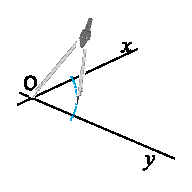
\includegraphics[width=2.4cm]{compasxOy} &  \includegraphics[width=2.4cm]{compas_arcsxOy} & \includegraphics[width=2.4cm]{bissectricexOy} \\ 
Au compas, on trace un arc de cercle de centre $O$ qui coupe chaque côté de l'angle en un point. & On trace deux arcs de cercle de même rayon ayant ces deux points pour centres. Ces arcs se coupent en un point. & La bissectrice de l'angle $\widehat{xOy}$ est la demi-droite d'origine $O$ passant par ce point. \\
\end{tabularx} \\

 \end{exemple*1}

\exercice 

Trace un triangle $ABC$ tel que $AB=4$\,cm ; $AC=7$\,cm ; $BC=5$\,cm ; puis trace les bissectrices des angles $\widehat{ABC}$ ; $\widehat{BAC}$ et $widehat{ACB}$. Que remarques-tu ?

%\correction

 
\end{methode*1}

%%%%%%%%%%%%%%%%%%%%%%%%%%%%%

\section{Le cercle}

\begin{definition}
Un \textbf{\MotDefinition{cercle}{}} de centre $O$ est l'ensemble des points situés à la même distance du point $O$. 
Cette distance est le \textbf{\MotDefinition{rayon}{}} du cercle.
\end{definition}

\begin{aconnaitre}
\begin{tabularx}{.95\linewidth}{|X|p{5cm}|p{3cm}|}
\hline
\multirow{5}{*}{\includegraphics[width=3.4cm]{cercleAFNME}}  & Le \textcolor{C2}{\textbf{centre}} d'un cercle est le point équidistant de tous les points qui constituent ce cercle. & Le point $O$ est le \textcolor{C2}{\textbf{centre}} du cercle $(\mathcal{C})$.\\ \cline{2-3}
 & Un \textcolor{J1}{\textbf{rayon}} d'un cercle est un segment ayant pour extrémités le centre et un point de ce cercle. & Le segment $[OA]$ est un  \textcolor{J1}{\textbf{rayon}} du cercle $(\mathcal{C})$.\\ \cline{2-3}
  & Un  \textcolor{H1}{\textbf{diamètre}} d'un cercle est un segment ayant pour extrémités deux points de ce cercle et contenant son centre. & Le segment $[EF]$ est un  \textcolor{H1}{\textbf{diamètre}} du cercle $(\mathcal{C})$.\\ \cline{2-3}
 & Une  \textcolor{PartieFonction}{\textbf{corde}} d'un cercle est un segment ayant pour extrémités deux points de ce cercle. & Le segment $[MN]$ est une  \textcolor{PartieFonction}{\textbf{corde}} du cercle $(\mathcal{C})$.\\ \cline{2-3}
 & Un  \textcolor{B2}{\textbf{arc de cercle}} est une portion de cercle comprise entre deux points de ce cercle. & La portion de cercle $\overset{\huge{\frown}}{MN}$ comprise entre $M$ et $N$ est un  \textcolor{B2}{\textbf{arc du cercle}} $(\mathcal{C})$.\\ \hline
  \end{tabularx}
 \end{aconnaitre}
  
  
 \begin{remarque}
 Par commodité de langage, on appelle « rayon » la longueur du rayon d'un cercle, et  on appelle « diamètre » la longueur de son diamètre.
  \end{remarque}
  
 \begin{remarque}
 Le diamètre d'un cercle est égal au double de son rayon.
  \end{remarque}

\newpage

\begin{methode*1}[Vocabulaire du cercle]

 \begin{exemple*1} \\[0.75em]
Trace le cercle de centre $T$ passant par le point $U$. \\[0.5em]

\begin{tabularx}{\linewidth}{X|X|X}
 \includegraphics[width=1.8cm]{pointsUT} &  \includegraphics[width=3.2cm]{compasUT} & \includegraphics[width=3.2cm]{cercleUT} \\ 
  & \multicolumn{1}{|p{3cm}|}{On pointe le compas sur le point $T$ et on écarte le compas jusqu'à ce que la mine soit sur le point $U$.} & On trace le cercle. \\
\end{tabularx} 

 \end{exemple*1}

\exercice 

Trace un rectangle $ABCD$ tel que $AB=6$\,cm et $BC=3$\,cm. Trace les segments $[AC]$ et $[BD]$. On appelle $O$ leur point d'intersection. Trace le cercle de centre $O$ passant par $A$. Que remarques-tu ?

%\correction

 
\end{methode*1}

%%%%%%%%%%%%%%%%%%%%%%%%%%%%%





\exercicesbase
\begin{colonne*exercice}

\serie{Points, segments et droites}

\begin{exercice}[Avec un quadrillage]
 \begin{center} \includegraphics[width=7.2cm]{quadrillage} \end{center}
 \begin{enumerate}
  \item En utilisant le quadrillage de ton cahier, place les points $A$, $B$, $C$ et $D$ comme sur la figure ci-dessus :
  \item Trace en bleu le segment $[AB]$ ;
  \item Trace en vert le segment d'extrémités $D$ et $C$ ;
  \item Trace en rouge la droite passant par $A$ et $C$ ;
  \item Trace en noir la demi-droite d'origine $D$ passant par $B$.
  \end{enumerate}
 \end{exercice}


\begin{exercice}[Appartient ou pas ?]
 \begin{center} \includegraphics[width=4.8cm]{droiteABECD} \end{center}
 Après avoir observé la figure, recopie et complète les pointillés avec $\in$ ou $\notin$ :
    \begin{colenumerate}{3}
     \item $B$ \ldots $[AC]$
     \item $D$ \ldots $[AB]$
     \item $E$ \ldots $[AD]$
     \item $B$ \ldots $[CA)$
     \item $D$ \ldots $[CA)$
     \item $E$ \ldots $[CE]$
     \end{colenumerate}
\end{exercice}


\begin{exercice}[À trouver]
 \begin{center} \includegraphics[width=6.5cm]{droiteFGHIJK}  \end{center}
 Parmi les points nommés sur la figure, indique ceux qui appartiennent à :
    \begin{colenumerate}{2}
     \item $[FK]$ ;
     \item $[IG)$ ;
     \item $[FJ]$ et à $[GK]$ ;
     \item $[GJ)$ mais pas à $[HJ]$ ;
     \item $[FG]$ ou à $[IJ)$ ;
     \item $[FH]$ et à $[JK]$.
     \end{colenumerate}
\end{exercice}


\begin{exercice}[Vrai ou faux ?]
 \begin{center} \includegraphics[width=4.6cm]{segmentsAB-CD}  \end{center}
 Observe cette figure composée de deux segments $[AB]$ et $[CD]$ sécants et indique pour chaque affirmation si elle est vraie ou fausse :
 \begin{enumerate}
  \item Les points $C$, $D$ et $M$ sont alignés ;
  \item $M$ est le point d'intersection des segments $[AB]$ et $[CD]$ ;
  \item $M$ est le milieu du segment $[AC]$ ;
  \item $M$ est un point du segment $[CD]$ ;
  \item $A$ appartient au segment $[MB]$ ;
  \item $M$ est le milieu du segment $[CD]$.
 \end{enumerate}
\end{exercice}


\begin{exercice}[Milieux]
\begin{enumerate} 
 \item Trace un segment $[RS]$ de longueur 4,8 cm et place son milieu $T$ ;
 \item Place un point $U$ qui ne soit pas aligné avec $R$ et $S$ ;
 \item Place le point $V$ tel que $T$ soit le milieu du segment $[UV]$.
 \end{enumerate}
\end{exercice}


\begin{exercice}[À construire]
\begin{enumerate} 
 \item Place trois points $A$, $B$ et $C$ non alignés ;
 \item Trace les segments $[BC]$ et $[AC]$ ;
 \item Marque le milieu $I$ du segment $[BC]$ et le milieu $J$ du segment $[AC]$ ;
 \item Trace le segment d'extrémités $B$ et $J$ ;
 \item Note $K$ le point d'intersection des segments $[AI]$ et $[BJ]$ ;
 \item Trace le segment $[AB]$ et place son milieu $L$. Trace enfin le segment $[CL]$. Que remarques‑tu ?
 \end{enumerate}
\end{exercice}


\begin{exercice}[À construire (bis)]
\begin{enumerate} 
 \item Place trois points $L$, $M$ et $N$ non alignés ;
 \item Place un point $A$ appartenant au segment $[LN]$ ;
 \item Place un point $B$ appartenant à la demi‑droite $[MN)$ mais n'appartenant pas au segment $[MN]$ ;
 \item Place le point $C$ aligné d'une part avec $A$ et $B$, et d'autre part avec $L$ et $M$.
 \end{enumerate}
\end{exercice}


\begin{exercice}[Bande dessinée]
 \begin{center} \includegraphics[width=4.3cm]{bande-dessinee}  \end{center}
Pour chaque étape de la bande dessinée, écris la consigne qui a été donnée, sans tenir compte des mesures.
\end{exercice}

%%%%%%%%%%%%%%%%%%%%%%%%%%%%%%%%%%%%%%%%%%%%%%%%%%%%%%%%%

\serie{Droites parallèles et perpendiculaires}

\begin{exercice}[Position de droites]
 \begin{center} \includegraphics[width=5.8cm]{mikado}  \end{center}
Observe la figure ci‑dessus et note sur ton cahier :
\begin{itemize}
 \item Le nom des droites qui \textbf{te semblent} perpendiculaires ;
 \item Le nom des droites qui sont sécantes mais non perpendiculaires ;
 \item Le nom des droites qui \textbf{te semblent} parallèles.
 \end{itemize}
\end{exercice}


\begin{exercice}[Position de droites $(bis)$]
 \begin{center} \includegraphics[width=7.3cm]{mikado2}  \end{center}
\begin{enumerate}
 \item Quelles sont les droites qui sont à coup sûr perpendiculaires ?
 \item Quelle semble être la position relative des droites $(BA)$ et $(GR)$ ?
 \end{enumerate}
\end{exercice}


\begin{exercice}[Quadrillage]
Reproduis une figure similaire à celle ci‑dessous. Trace, à la règle, la droite $d_1$ perpendiculaire à la droite $d$ passant par le point $M$ et la droite $d_2$ parallèle à la droite $d'$ passant par $M$.
\begin{center} \includegraphics[width=5.2cm]{quadrillage2}  \end{center}
\end{exercice}


\begin{exercice}[Constructions]
\begin{enumerate}
 \item Reproduis sur une feuille blanche les deux figures ci‑dessous :
 \begin{center} \includegraphics[width=6.1cm]{constructions}  \end{center}
 \item Pour chacune des figures, trace :
  \begin{itemize}
   \item La droite $d'$ perpendiculaire à $d$ et passant par $B$ ;
   \item La droite $d''$ perpendiculaire à $d$ et passant par $A$.
   \end{itemize}
 \item Que peux‑tu dire des droites $d'$ et $d''$ ?
 \end{enumerate}
\end{exercice}


\begin{exercice}[Constructions $(bis)$]
 \begin{center} \includegraphics[width=5.7cm]{constructions2}  \end{center}
\begin{enumerate}
 \item Reproduis la figure ci‑dessus ;
 \item Trace $d'$, la parallèle à $d$ passant par $A$ ;
 \item Trace $d''$, la parallèle à $d$ passant par $B$ ;
 \item Que peux‑tu dire des droites $d'$ et $d''$ ?
 \end{enumerate}
\end{exercice}


\begin{exercice}[Programme de construction]
\begin{enumerate}
 \item Place deux points $A$ et $B$ tels que $AB = 8$ cm ;
 \item Place un point $L$ sur $[AB]$ tel que $AL = 3$ cm ;
 \item Trace la droite $d$ telle que $L \in d$ et $(AB) \perp d$ ;
 \item Place un point $C$ tel que $C \in d$ et $LC = 2$ cm ;
 \item Trace la droite $d'$ telle que $d' \parallel (AB)$ et $C \in d'$ ;
 \item Sur la demi‑droite $[BC)$, place le point $I$ tel que $BI = 7$ cm ;
 \item Trace la droite $d''$ telle que $I \in d''$ et $d'' \parallel (AC)$.
 \end{enumerate}
\end{exercice}


\begin{exercice}
Construis la figure suivante : \\[0.75em]
\begin{minipage}[c]{0.2\textwidth}
\includegraphics[width=3.8cm]{constructions3}
 \end{minipage} \hfill%
 \begin{minipage}[c]{0.2\textwidth}
 $(BM) \parallel (AN)$
  \end{minipage} \\
\end{exercice}


\begin{exercice}
Reproduis la figure ci‑dessous en vraie grandeur : \\[0.75em]
\begin{minipage}[c]{0.2\textwidth}
\includegraphics[width=4.5cm]{double-triangle}
 \end{minipage} \hfill%
 \begin{minipage}[c]{0.2\textwidth}
$AB = 5,3$ cm ;
$BC = 3$ cm ;
$AC = 7,7$ cm.
 \end{minipage} \\
\end{exercice}

%%%%%%%%%%%%%%%%%%%%%%%%%%%%%%%%%%%%%%%%%%%%%%%%%%%%%%%%%

\serie{Médiatrice d’un segment}

\begin{exercice}[Médiatrices]
Dans chaque cas, trace le segment de longueur donnée puis sa médiatrice :
 \begin{colenumerate}{3}
  \item $AB = 2$ cm 
  \item $DE = 7,8$ cm
  \item $FG = 76$ mm
  \end{colenumerate}
\end{exercice}


\begin{exercice}[Points alignés]
 \begin{enumerate}
  \item Trace un segment $[AB]$ de longueur 7 cm ;
  \item Place le point $C$ de la demi‑droite $[BA)$ tel que $BC = 12$ cm ;
  \item Construis la médiatrice $m_1$ du segment $[AC]$ ;
  \item Construis la médiatrice $m_2$ du segment $[AB]$ ;
  \item Que remarques‑tu ?
  \end{enumerate}
\end{exercice}


\begin{exercice}[Reconnaître]
Sur chacune des figures ci‑dessous, indique si $P$ est sur la médiatrice de $[AB]$ : \\[0.5em]
 \begin{colenumerate}{2}
  \item 
  
  \includegraphics[width=2.2cm]{mediatriceAB1}
  \item 
  
  \includegraphics[width=2.2cm]{mediatriceAB2}
  \item 
  
  \includegraphics[width=2.2cm]{mediatriceAB3}
  \item 
  
  \includegraphics[width=2.2cm]{mediatriceAB4}
  \end{colenumerate}
\end{exercice}
 
 
\begin{exercice}[Construction]
 \begin{enumerate}
 \item Trace un segment $[AB]$ de longueur 6 cm ;
 \item Construis la médiatrice $d$ du segment $[AB]$ au compas ;
 \item Place un point $M$ sur $d$ à 7 cm de $A$ ;
 \item Quelle est la longueur de $[BM]$ ? 
 
Tu la justifieras en utilisant une propriété.
  \end{enumerate}
\end{exercice}


\begin{exercice}[Concours de médiatrices]
 \begin{enumerate}
 \item Place trois points $A$, $B$ et $C$ non alignés.
 \item Trace sans équerre les médiatrices des segments $[AB]$, $[AC]$ et $[BC]$. 
 
 Que constates‑tu ?
 \end{enumerate}
\end{exercice}

%%%%%%%%%%%%%%%%%%%%%%%%%%%%%%%%%%%%%%%%%%%%%%%%%%%%%%%%%

\serie{Cercle}

\begin{exercice}[Vocabulaire]
 \begin{center} \includegraphics[width=2.1cm]{cercleABC} \end{center}
 Sur la figure ci-dessus : 
 
$A$, $B$ et $C$ sont sur le cercle de centre $O$ ;

$A$, $O$ et $B$ sont alignés.
 \begin{enumerate}
  \item Écris deux phrases décrivant la figure, en utilisant les mots « rayon » et « diamètre » ;
  \item Recopie et complète les phrases suivantes :
   \begin{itemize}
    \item Le point $O$ est le milieu du \ldots \ldots \ldots ;
    \item Le point $O$ est une extrémité du \ldots \ldots \ldots ;
    \item $A$ et $B$ sont les \ldots \ldots \ldots du \ldots \ldots \ldots $[AB]$ ;
    \item La portion de cercle comprise entre les points $A$ et $C$ est l'\ldots \ldots \ldots.
    \end{itemize}
  \end{enumerate}
\end{exercice}


\begin{exercice}[Avec le rayon]
Trace un cercle de centre $O$ et de rayon 4 cm puis un cercle de rayon 4 cm et passant par $O$.
\end{exercice}


\begin{exercice}[Avec le diamètre]
 \begin{enumerate}
  \item Trace un segment $[AB]$ de longueur 5 cm ;
  \item Trace le cercle de diamètre $[AB]$ ;
  \item Quelle est la mesure du rayon de ce cercle ?
  \end{enumerate}
\end{exercice}


\begin{exercice}[Construction]
 \begin{enumerate}
  \item Trace un cercle $(\mathcal{C})$ de centre $O$ et de rayon 4,5 cm ;
  \item Place un point $A$ sur le cercle $(\mathcal{C})$ et place le point $B$ diamétralement opposé au point $A$.
  \item Marque un point $D$ à l'extérieur du cercle $(\mathcal{C})$ et trace le cercle de diamètre $[BD]$.
 \end{enumerate}
\end{exercice}


\begin{exercice}[Calculs]
 \begin{enumerate}
  \item Trace un segment $[AB]$ de longueur 6 cm. Trace le cercle de centre $A$ et de rayon 2 cm. Ce cercle coupe la droite $(AB)$ en deux points $M$ et $N$. On appelle $M$ celui qui appartient au segment $[AB]$ ;
  \item Calcule les longueurs $BM$ et $BN$.
 \end{enumerate}
\end{exercice}


\begin{exercice}[Concentriques]
Deux cercles concentriques (c'est‑à‑dire de même centre) $\mathcal(C)$ et $\mathcal(C’)$ ont pour centre $O$ et pour rayons respectifs 3 cm et 5 cm. $[GH]$ est un diamètre du cercle $\mathcal(C)$. 

La droite passant par $G$ et par $H$ coupe le cercle $\mathcal(C’)$ en deux points $I$ et $J$ ; on appelle $I$ celui qui est le plus près de $G$.
\begin{enumerate}
  \item Fais une figure ;
  \item Calcule les longueurs $GI$ et $JG$.
 \end{enumerate}
\end{exercice}


\begin{exercice}[Calculs]
\begin{enumerate}
  \item Trace un segment $[ST]$ de longueur 6 cm. Sur ce segment, marque le point $U$ tel que $SU = 3,2$ cm. Trace le cercle $\mathcal(C)$ de centre $T$ et qui passe par $U$ ;
  \item Calcule le diamètre du cercle $\mathcal(C)$ ;
  \item Sur le segment $[UT]$, place le point $V$ tel que $UV = 1,2$ cm. Quel est le rayon du cercle de diamètre $[SV]$ ?
 \end{enumerate}
\end{exercice}


\begin{exercice}
Construis la figure ci-dessous donnée par son croquis.

\begin{center} \includegraphics[width=3.4cm]{double-cercle} \end{center}
\end{exercice}


\begin{exercice}
Construis chaque figure ci-dessous donnée par son croquis.
\begin{colenumerate}{2}
 \item
 
 \includegraphics[width=3.9cm]{4cercles}
 \item
 
\includegraphics[width=2.6cm]{goutte-rose}
 \item
 
\includegraphics[width=4cm]{theatre}
 \end{colenumerate}
\end{exercice}


\begin{exercice}
En utilisant le quadrillage de ton cahier, reproduis les figures suivantes.
\begin{colenumerate}{2}
 \item
 
 \includegraphics[width=2.9cm]{quadrillage-cercles}
 \item
 
\includegraphics[width=3.1cm]{quadrillage-parap}

 \end{colenumerate}
\end{exercice}


\begin{exercice}
Recopie et complète le programme de construction de la figure ci‑dessous :
\begin{center}  \includegraphics[width=3.6cm]{cercle-triangle} \end{center}
\begin{itemize}
 \item Trace un cercle de \ldots \ldots $O$ et de \ldots \ldots 2,4 cm ;
 \item Trace un \ldots \ldots $[AB]$ de ce cercle ;
 \item Trace une \ldots \ldots $[AM]$ telle que $AM =$ \ldots \ldots ;
 \item Place le point $C$ tel que $M$ soit le \ldots \ldots de $[AC]$ ;
 \item Trace le \ldots \ldots $[CB]$.
 \end{itemize}
\end{exercice}


\begin{exercice}[À construire]
\begin{enumerate}
 \item Trace un segment $[AB]$ de longueur 6 cm ;
 \item Marque le point $O$, milieu du segment $[AB]$ ;
 \item Trace le cercle de centre $O$ et de rayon 3 cm ;
 \item Trace les cercles de diamètres $[AO]$ et $[OB]$.
 \end{enumerate}
\end{exercice}


\begin{exercice}[À construire $(bis)$]
\begin{enumerate}
 \item Trace un segment $[AB]$ de longueur 9 cm ;
 \item Trace le cercle de centre $A$ et de rayon 3 cm. On appelle $C$ le point d'intersection de ce cercle et du segment $[AB]$ ;
 \item Trace le cercle de centre $B$ et de rayon 3 cm. Il coupe le segment $[AB]$ en $D$ ;
 \item Trace un demi‑cercle de diamètre $[CD]$.
 \end{enumerate}
\end{exercice}


\begin{exercice}
Écris un programme de construction pour chacune des figures suivantes.

\begin{colenumerate}{1}
 \item 
 
 \includegraphics[width=3.3cm]{double-cercle2}
 \item 

\includegraphics[width=5.3cm]{cercle-triangle2}
 \end{colenumerate}
\end{exercice}


%%%%%%%%%%%%%%%%%%%%%%%%%%%%%%%%%%%%%%%%%%%%%%%%%%%%%%%%%

\serie{Nommer un angle}


\begin{exercice}[De toutes les couleurs]
Les points $A$, $O$ et $L$ sont alignés.
 \begin{center} \includegraphics[width=6.7cm]{angles-colores}  \end{center}
\begin{enumerate}
 \item Nomme les angles marqués en couleur dans la figure de toutes les façons possibles ; 
 \item Reproduis la figure puis marque en bleu l'angle $\widehat{yOz}$ en rouge l'angle $\widehat{PMC}$ et en vert l'angle $\widehat{PAL}$.
 \end{enumerate}
\end{exercice}


\begin{exercice}[Plusieurs noms]
Les segments $[TD]$ et $[PS]$ sont sécants en $A$ et les segments $[PI]$ et $[TD]$ se coupent en $R$.

Trouve toutes les autres façons de nommer : \\[0.5em]
\begin{minipage}[c]{0.2\textwidth}
\begin{itemize}
 \item l'angle $\widehat{APR}$ ;
 \item l'angle $\widehat{RDI}$ ;
 \item l'angle $\widehat{PDA}$.
 \end{itemize}
 \end{minipage} \hfill%
  \begin{minipage}[c]{0.4\textwidth}
  \includegraphics[width=4.7cm]{segments-secants}
  \end{minipage} \\
\end{exercice}  


\begin{exercice}[Quelle étourdie !]
Louise a recopié la figure ci‑dessous qui était au tableau mais elle a oublié de noter les noms des points d'intersection des droites. 
 \begin{center} \includegraphics[width=5.2cm]{angles-multicolores}  \end{center}
Elle appelle son camarade Ahmed qui lui dit que les angles en couleur se nomment $\widehat{ABC}$, $\widehat{DBA}$, $\widehat{FAC}$ et $\widehat{FAE}$.

Reproduis la figure et nomme les points grâce à ces indications.
\end{exercice}  


%%%%%%%%%%%%%%%%%%%%%%%%%%%%%%%%%%%%%%%%%%%%%%%%%%%%%%%%%

\serie{Mesure d'un angle}


\begin{exercice}[À vue d’œil]
Indique les angles qui te paraissent obtus, aigus ou droits.
 \begin{center} \includegraphics[width=7cm]{angles-toutgenre}  \end{center}
\end{exercice}


\begin{exercice}[Avec l'équerre]
En utilisant ton équerre, détermine quels sont les angles aigus, obtus ou droits dans chacun des cas ci-dessous.
 \begin{center} \includegraphics[width=7cm]{angles-droits}  \end{center}
\end{exercice}


\begin{exercice}[Bien placé ?]
Dans chacun des cas suivants, José souhaite mesurer l'angle $\widehat{BAC}$.

Peut‑il effectuer une mesure correcte ? Si oui, indique la mesure de l'angle et si non, explique pourquoi. \\[0.5em]
\begin{colenumerate}{2}
 \item 
 
 \includegraphics[width=3.6cm]{rapporteurA}
 \item 
 
  \vspace{-2em} \includegraphics[width=3.6cm]{rapporteurB}
 \item 
 
 \includegraphics[width=3.6cm]{rapporteurC}
 \item 
 
 \includegraphics[width=3.6cm]{rapporteurD}
 \item 
 
 \includegraphics[width=3.6cm]{rapporteurE}
 \item 
 
 \vspace{-2em} \includegraphics[width=3.6cm]{rapporteurF}
 \end{colenumerate}
\end{exercice}  
\end{colonne*exercice}


\exercicesappr
\begin{colonne*exercice}

\begin{exercice}[Pirates et équidistance]
Les pirates Olivier Levasseur et Anne Bonny se disputent un diamant. Jo l'intello cherche une méthode équitable pour savoir qui aura la pierre précieuse. Reproduis précisément les parchemins que dessine Jo, au fur et à mesure de la discussion.
\begin{enumerate}
 \item « Vous n'avez qu'à vous placer à 50 pas l'un de l'autre, et mettre le diamant au milieu ». 
 
Il fait un premier dessin sur un parchemin pour schématiser sa proposition, en représentant 10 pas par 1 centimètre.
 \item Les pirates estimant que la course n'est pas assez longue pour les départager, Jo propose un second schéma : « Vous vous mettez toujours à 50 pas l'un de l'autre, mais vous mettez le diamant à 70 pas de chacun de vous. Je me placerai au milieu de vous deux. ». \\[-0.9em]
 \item Jo réfléchit, puis propose un troisième schéma : « On n'a qu'à se mettre tous les trois à 70 pas du diamant et vous vous placerez à 100 pas de moi ».
 \end{enumerate}
\end{exercice} 


\begin{exercice}[À partir d'une figure $(bis)$]
On considère la figure suivante :
\begin{center} \includegraphics[width=5.8cm]{droites-sec-paral} \end{center}
On donne de plus : $d_1 \parallel d_2$ et $d_4 \parallel d_6$.
 \begin{enumerate}
  \item Reproduis cette figure et ajoute tous les angles droits possibles.
  \item Quelles sont les droites parallèles à $d_3$ ?
  \item Quelles sont les droites parallèles à $d_6$ ?
  \item Quelles sont les droites sécantes à $d_7$ ?
  \end{enumerate}
\end{exercice}


\begin{exercice}[Partage équitable]
Marie organise une soirée avec cinq de ses amis. Ils achètent une pizza et une tarte, toutes deux de forme circulaire.
\begin{enumerate}
 \item Comment doit procéder Marie pour partager équitablement sa pizza avec ses amis ?
 \item Au moment du dessert, ses parents, son frère et sa sœur se joignent à la petite fête. Marie doit découper la tarte équitablement. Comment procède‑t‑elle ?
 \end{enumerate}
\end{exercice}


\begin{exercice}[Des histoires de milieux]
Construis $d_1$ et $d_2$ deux droites perpendiculaires en $O$. $A$ est un point de $d_1$ et $B$ un point de $d_2$. $C$ est le point de $d_1$ tel que $O$ soit le milieu de $[AC]$ et $D$ le point de $d_2$ tel que $O$ soit le milieu de $[BD]$.
\begin{enumerate}
 \item Que représente $d_1$ pour $[BD]$ ? Et $d_2$ pour $[AC]$ ? Justifie tes réponses.
 \item Place $I$ le milieu de $[AB]$ et $I'$ le point de $(OI)$ tel que $O$ soit le milieu de $[II']$.
 \item Où semble être placé le point $I'$ ?
 \item Comment semblent être les droites $(AD)$, $(II')$ et $(BC)$ ?
 \end{enumerate}
\end{exercice}


\begin{exercice}
Voici le croquis d'un pilier réalisé par un architecte.
\begin{center} \includegraphics[width=3.9cm]{pilier} \end{center}
Construis ce pilier à l’échelle suivante : 3 cm sur la figure représentent 1 m dans la réalité.
\end{exercice}


\begin{exercice}[Orion]
Alex observe la constellation d'Orion dans le ciel au travers de son télescope. Il voudrait la représenter pour son prochain exposé. Pour cela, il réalise quelques mesures ; il a reporté ses observations sur le croquis ci‑dessous.

Construis pour Alex la constellation d'Orion.
\begin{center} \includegraphics[width=7.1cm]{orion1} \end{center}
\begin{center} $\boxed{\includegraphics[width=4cm]{orion2}}$ 

{\footnotesize\emph{La constellation d'Orion.}} \end{center}
\end{exercice}
\end{colonne*exercice}

\connaissances
\begin{acquis}
\begin{itemize}
\item BlaBla1
\item BlaBla2
\item BlaBla3
\item BlaBla4
\item BlaBla5
\item BlaBla6
\end{itemize}
\end{acquis}

\QCMautoevaluation{Pour chaque question, plusieurs réponses sont
  proposées.  Déterminer celles qui sont correctes.} % Est-ce que c'est toujours le cas ?

\begin{QCM}
  \begin{GroupeQCM} % Est-ce qu'on les séparent en groupe ?
    \begin{exercice}
      Quelle est la bonne réponse ?
      \begin{ChoixQCM}{4}
      \item un
      \item deux
      \item trois
      \end{ChoixQCM}
\begin{corrige}
     \reponseQCM{ab} % ici deux réponses justes
   \end{corrige}
    \end{exercice}


\end{GroupeQCM}
\end{QCM}

  

\TravauxPratiques % pour nous "travailler en groupe"

\begin{TP}[]

Mon super TP

\end{TP}



\pagebreak

\Recreation
%\input{PointsSegmentsDroites/PtSegDr_fin_chap.tex}


